\documentclass[12pt]{article}
\usepackage[utf8]{inputenc}
\usepackage{amsmath}

\title{ECE 3413 Lab 03\\*Linear Time Invariant (LTI) system\\* and LTI transfer function}
\author{Leomar Dur\'an}
\date{$8^{\text{th}}$ February 2023}

\usepackage{hyperref}

\usepackage[per-mode=symbol]{siunitx}
\usepackage{xfrac}
\usepackage{amssymb}
\newcommand*\transpose{\mathsf{T}}

\usepackage{mathtools}%
\DeclarePairedDelimiter\brao()%
\DeclarePairedDelimiter\brac[]%
\DeclarePairedDelimiter\braco[)%
\DeclarePairedDelimiter\Brac\{\}%
\DeclarePairedDelimiter\norm\lVert\rVert%
\DeclarePairedDelimiter\piecefn\{.
\DeclarePairedDelimiter\evalat.|

\usepackage{lib/nonfloatenvirons}
\usepackage{booktabs}
\newcommand\ra[1]{\renewcommand*\arraystretch{#1}}
\ra{1.25}
\usepackage{minted}

\usepackage{adjustbox}
\newcommand*\mcadj[7]%
% {#columns}{col spec}{rotation}{adjust spec}
% {before rotated text}{rotated text}{after rotated text}
{%
    \multicolumn{#1}{#2}{%
        \rlap{%
            #5\adjustbox{rotate=#3,#4}{#6}~#7%
        }%
    }%
}

\usepackage{pdfpages}
\usepackage{standalone}
\usepackage{matlab}

% \newcommand*\matlabtitle\subsection
% \newcommand*\matlabheading\subsubsection
% \newcommand*\mlcell[1]{#1}
% \newenvironment{matlaboutput}{%
    % \minted{matlab}%
% }%
% {%
    % \endminted%
% }%
% \newenvironment{matlabtableoutput}{}{}%

\def\hr{{\par\noindent\rule{\textwidth}{0.4pt}}}

\begin{document}

\maketitle
\newpage

\section{Introduction}

The purpose of this experiment is to serve as a practical introduction to Matlab and Simulink and their graphical user interface.

Matlab is a linear algebra tool, and Simulink is a tool for modeling systems using block diagrams.
They may each be used for modeling control systems among other types of systems.

In this example, we use Matlab to model a polynomial as a row vector of coefficients.
We also use Matlab in conjunction with Simulink to prepare, model and contrast $2$ control systems.

\section{Procedure}

\subsection{A translational mechanical system}

\begin{figure}[h]
    \centering
    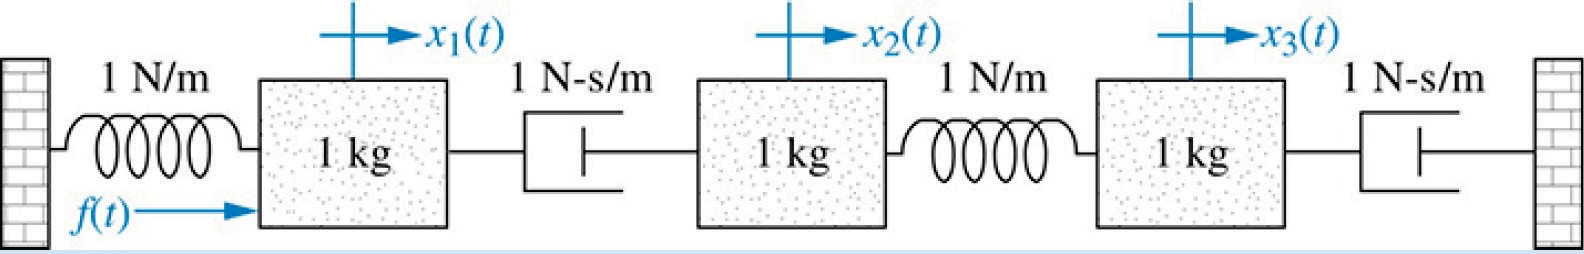
\includegraphics[width=\linewidth]{part01_translational_mechanical_system.png}
    \caption{Diagram of the translational mechanical system.}
    \label{fig:translational mechanical system}
\end{figure}

A state-space representation is a mathematical model of a physical system using variables that are in the time domain.

We are given the translational mechanical system
in Fig. \ref{fig:translational mechanical system}
that outputs $x_3\brao*t$.
From this system, let's define masses
\begin{equation}
    \vec{M} := \brac*{
        \begin{matrix} M_1 & M_2 & M_3 \end{matrix}
    }^\transpose = \brac*{
        \begin{matrix} \SI1{\kilo\gram} & \SI1{\kilo\gram} & \SI1{\kilo\gram} \end{matrix}
    }^\transpose\rlap,
\end{equation}
spring constants
\begin{equation}
    \vec{K} := \brac*{
        \begin{matrix} K_1 & K_2 \end{matrix}
    }^\transpose = \brac*{
        \begin{matrix} \SI1{\newton\per\meter} & \SI1{\newton\per\meter} \end{matrix}
    }^\transpose\rlap,
\end{equation}
and damping constants
\begin{equation}
    \vec{D} := \brac*{
        \begin{matrix} D_1 & D_2 \end{matrix}
    }^\transpose = \brac*{
        \begin{matrix} \SI1{\newton\second\per\meter} & \SI1{\newton\second\per\meter} \end{matrix}
    }^\transpose\rlap.
\end{equation}

\subsubsection{Free body diagram}
This system has the free body diagram shown in the CAD drawing on the following page.
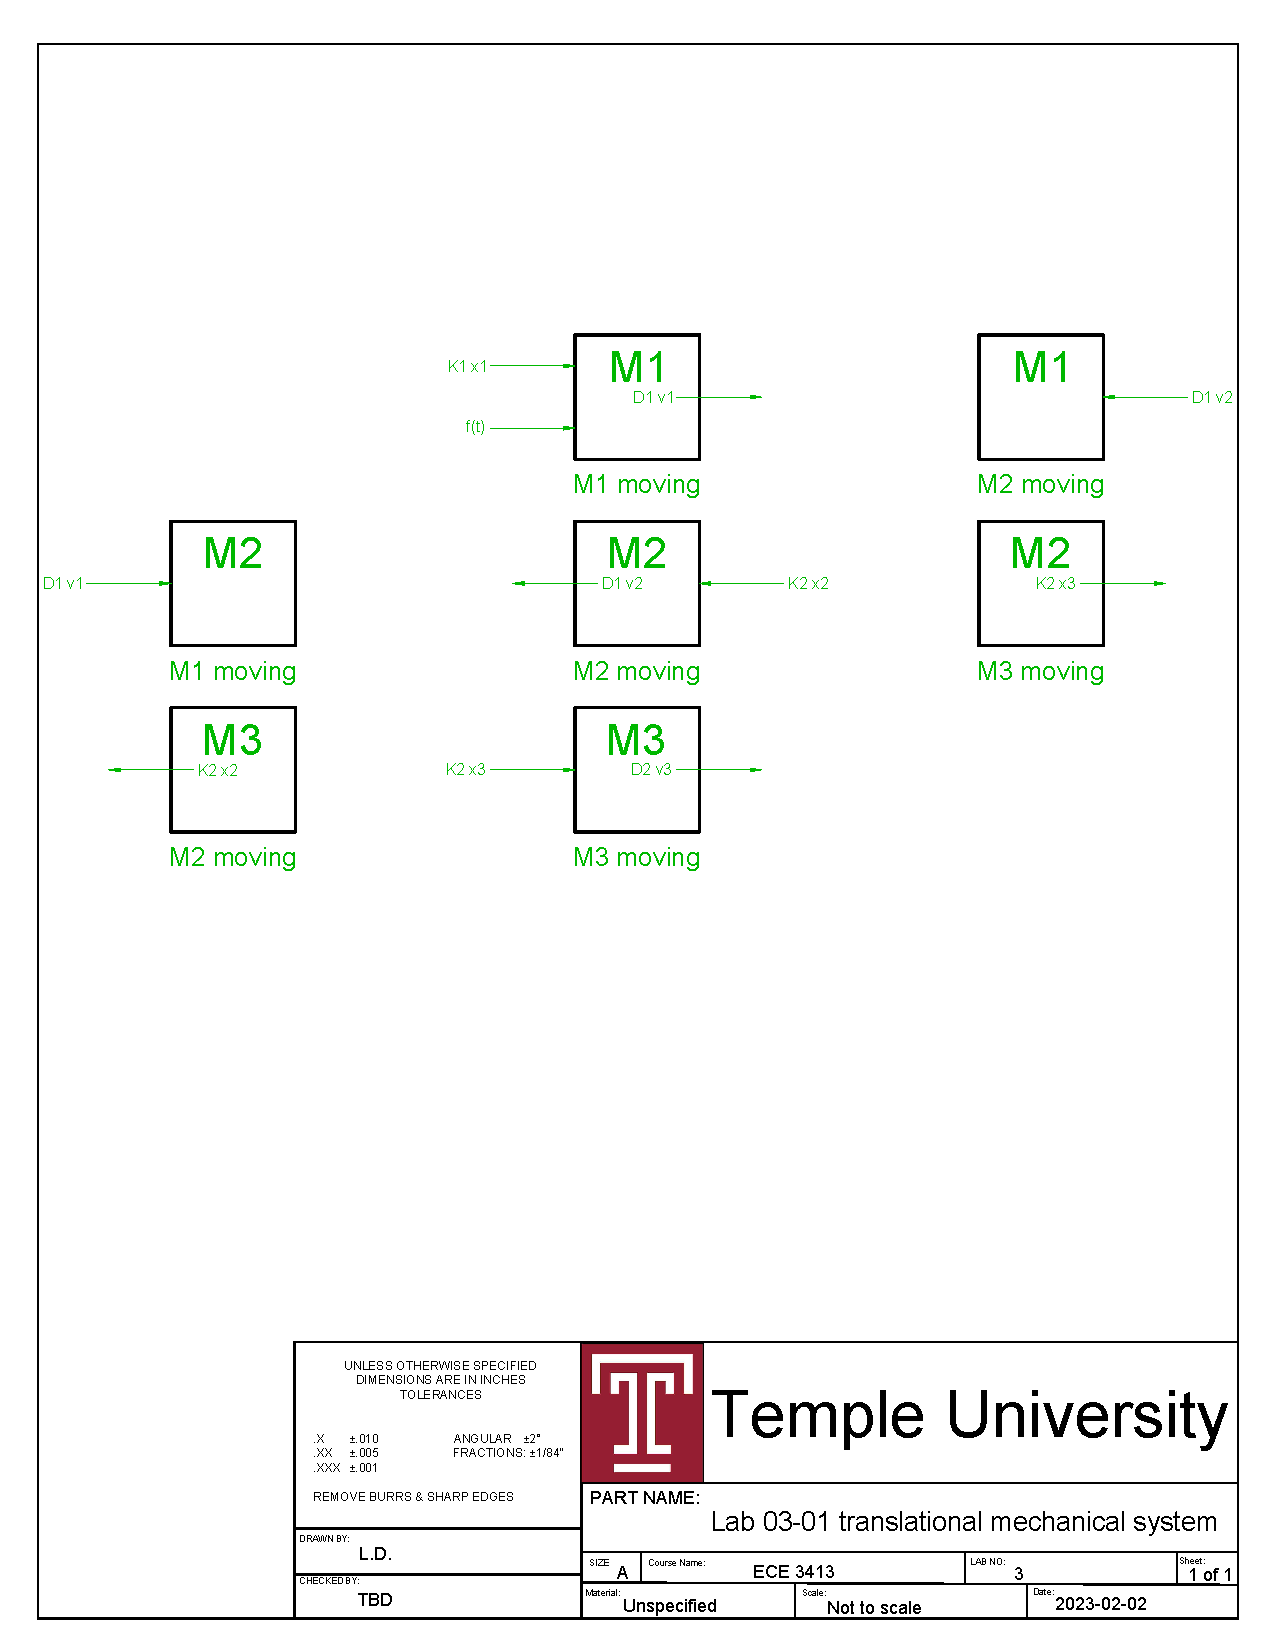
\includepdf{lab03-01 translational mechanical system fbd-A size.pdf}

\subsubsection{Mathematical state-space representation}

Then we find the total force at each mass applying superposition for each possible state.

\begin{equation}
    \piecefn*{
        \begin{array}{@{}l@{}}
            M_1 \ddot{x}_1 = \sum F_{M1\mathrm{x}} = K_1 x_1 + f\brao*t + D_1 \brao*{\dot{x}_1 - \dot{x}_2}\rlap,
        \\*
            M_2 \ddot{x}_2 = \sum F_{M2\mathrm{x}} = D_1\brao*{\dot{x}_1 - \dot{x}_2} + K_2\brao*{-x_2 + x_3}\rlap,
        \\*
            M_3 \ddot{x}_3 = \sum F_{M3\mathrm{x}} = K_2\brao*{-x_2 + x_3} + D_2\dot{x}_3\rlap.
        \\*
        \end{array}
    }
\end{equation}

Next, we relate states $\underline{\hat{x}} \in \mathbb{R}^6$ to position as in Table \ref{tab:states to position}.

\begin{table}[h]
    \centering
    \caption{How states relate to the position variables}
    \[
        \begin{array}{@{}r@{}c@{}l@{}}
        \toprule
            \text{state} & & \text{position}
        \\*
        \midrule
            {\hat{x}}_1 &{}={}& \dot{x}_1\rlap,
        \\*
            {\hat{x}}_2 &{}={}& x_1\rlap,
        \\*
            {\hat{x}}_3 &{}={}& \dot{x}_2\rlap,
        \\*
            {\hat{x}}_4 &{}={}& x_2\rlap,
        \\*
            {\hat{x}}_5 &{}={}& \dot{x}_3\rlap,
        \\*
            {\hat{x}}_6 &{}={}& x_3\rlap.
        \\*
        \bottomrule
        \end{array}
    \]
    \label{tab:states to position}
\end{table}

Thus, we can the derivatives of the states to the states with
the output $y := x_3 = {\hat{x}}_6$ represented by the first row
and using
the force equations for even rows, representing accelerations,
and the state--position relations for odd rows after the first, representing velocities,
giving the state-space representation

\begin{equation}
    \begin{array}{*4{@{}c}@{}}
            \mcadj1{@{}c@{}}{45}{}{\phantom{$=$}}{$
                = \brac*{
                    \begin{array}{@{}c@{}}
                        y
                    \\*
                    \midrule
                        \dot{\underline{\hat{x}}}
                    \\*
                    \end{array}
                }
            $}{}
        & &
            \mcadj1{@{}c@{}}{45}{}{\phantom{$=$}}{$
                =: \brac*{
                    \begin{array}{@{}c|c@{}}
                             D & \mathbf{C}
                    \\*
                    \midrule
                        \vec{B} & \mathbf{A}
                    \\*
                    \end{array}
                }
            $}{}
        &
            \mcadj1{@{}c@{}}{45}{}{\phantom{$=$}}{$
                = \brac*{
                    \begin{array}{@{}c@{}}
                        f
                    \\*
                    \midrule
                        \underline{\hat{x}}
                    \\*
                    \end{array}
                }
            $}{}
    \\*
        \brac*{
            \begin{array}{@{}c@{}}
                y \\*
            \midrule
                \dot{\hat{x}}_1 \\* \dot{\hat{x}}_2 \\*
                \dot{\hat{x}}_3 \\* \dot{\hat{x}}_4 \\*
                \dot{\hat{x}}_5 \\* \dot{\hat{x}}_6 \\*
            \end{array}
        }
        &{}={}&
        \brac*{
            \begin{array}{@{}c|*6c@{}}
                0 & 0 & 0 & 0 & 0 & 0 & 1
            \\*
            \midrule
                \sfrac1{M_1} & \sfrac{+D_1}{M_1} & \sfrac{K_1}{M_1} & \sfrac{-D_1}{M_1} & 0 & 0 & 0
            \\*
                0 & 1 & 0 & 0 & 0 & 0 & 0
            \\*
                0 & \sfrac{+D_1}{M_2} & 0 & \sfrac{-D_1}{M_2} & \sfrac{-K_2}{M_2} & 0 & \sfrac{+K_2}{M_2}
            \\*
                0 & 0 & 0 & 1 & 0 & 0 & 0
            \\*
                0 & 0 & 0 & 0 & \sfrac{-K_2}{M_3} &  \sfrac{D_2}{M_3} & \sfrac{+K_2}{M_3}
            \\*
                0 & 0 & 0 & 0 & 0 & 1 & 0
            \\*
            \end{array}
        }
        &
        \brac*{
            \begin{array}{@{}c@{}}
                f \\*
            \midrule
                {\hat{x}}_1 \\* {\hat{x}}_2 \\*
                {\hat{x}}_3 \\* {\hat{x}}_4 \\*
                {\hat{x}}_5 \\* {\hat{x}}_6 \\*
            \end{array}
        }.
    \end{array}
\end{equation}

\subsubsection{State-space representation in Matlab}

We can use the Matlab function \mintinline{matlab}{ss} to create a state-space representation object.
This function accepts the matrices of coefficients $\mathbf{A}$, $\vec{B}$, $\mathbf{C}$ and $D$ and returns a transfer function in state-space representation form.

This is a transfer function, just like the rational of polynomials \mintinline{matlab}{tf} and zero/pole/gain form \mintinline{matlab}{zpk}.
The $3$ types of objects are mutually convertible,
by using the target class's function on any transfer function object.

\subsection{Rational of polynomials form}

\subsubsection{Conversion using Matlab}

As stated in the previous section,
we may use the \mintinline{matlab}{tf} to convert from the state-space representation to the rational of polynomials form
just as we have with the zero/pole/gain form.
This gives us the transfer function
\begin{equation}
    T\brao*s = \brao*{\frac{x_3}{F}}\brao*s.
\end{equation}

\subsubsection{Equation for the transfer function}

Given a translational mechanical system with $m$ masses in movement,
we may find the transfer function using the equation
\begin{equation}
    T\brao*s = \mathbf{C}\brao*{s\mathbf{I}_{\brao*{2m}} - \mathbf{A}}\vec{B}
\end{equation}

We use Matlab to calculate the result and compare it to the converted transfer function.

\section{Results}

\hr

% This LaTeX was auto-generated from MATLAB code.
% To make changes, update the MATLAB code and export to LaTeX again.

\documentclass{article}

\usepackage[utf8]{inputenc}
\usepackage[T1]{fontenc}
\usepackage{lmodern}
\usepackage{graphicx}
\usepackage{color}
\usepackage{hyperref}
\usepackage{amsmath}
\usepackage{amsfonts}
\usepackage{epstopdf}
\usepackage[table]{xcolor}
\usepackage{matlab}

\sloppy
\epstopdfsetup{outdir=./}
\graphicspath{ {./part01_translational_mechanical_system_mlx_images/} }

\begin{document}

\matlabtitle{Part 1 $-$ Translational mechanical system}


\matlabheading{As a state-space model}

\begin{par}
\begin{flushleft}
is represented by the matrices of coefficients
\end{flushleft}
\end{par}

\begin{matlaboutput}
Mssr =
 
  A = 
       x1  x2  x3  x4  x5  x6
   x1   1   1  -1   0   0   0
   x2   1   0   0   0   0   0
   x3   1   0  -1  -1   0   1
   x4   0   0   1   0   0   0
   x5   0   0   0  -1   1   1
   x6   0   0   0   0   1   0
 
  B = 
       u1
   x1   1
   x2   0
   x3   0
   x4   0
   x5   0
   x6   0
 
  C = 
       x1  x2  x3  x4  x5  x6
   y1   0   0   0   0   0   1
 
  D = 
       u1
   y1   0
 
Continuous-time state-space model.
\end{matlaboutput}
\end{document}


\ \hr \\*

% This LaTeX was auto-generated from MATLAB code.
% To make changes, update the MATLAB code and export to LaTeX again.

\documentclass{article}

\usepackage[utf8]{inputenc}
\usepackage[T1]{fontenc}
\usepackage{lmodern}
\usepackage{graphicx}
\usepackage{color}
\usepackage{hyperref}
\usepackage{amsmath}
\usepackage{amsfonts}
\usepackage{epstopdf}
\usepackage[table]{xcolor}
\usepackage{matlab}

\sloppy
\epstopdfsetup{outdir=./}
\graphicspath{ {./part02_ratio_of_polynomials_form_mlx_images/} }

\begin{document}

\matlabtitle{Part 2 $-$ Rational of polynomials form}


\matlabheading{1. Conversion using Matlab}

\begin{par}
\begin{flushleft}
The transfer function from the state-space representation
\end{flushleft}
\end{par}

\begin{matlaboutput}
Mtf =
 
                   -s + 2.768e-16
  -------------------------------------------------
  s^6 - s^5 - s^4 - 2 s^3 + 2 s^2 + 2 s + 2.053e-16
 
Continuous-time transfer function.
\end{matlaboutput}

\matlabheading{2. Equation for transfer functions}

\begin{par}
\begin{flushleft}
create a transfer function that is just s
\end{flushleft}
\end{par}

\begin{matlaboutput}
T =
 
                   -s - 1.371e-16
  -------------------------------------------------
  s^6 - s^5 - s^4 - 2 s^3 + 2 s^2 + 2 s - 2.435e-16
 
Continuous-time transfer function.
\end{matlaboutput}

\matlabheading{Coefficient of determination $R^2$}

\begin{par}
\begin{flushleft}
To compare the transfer functions, let's find the $R^2$ value of all coefficients.
\end{flushleft}
\end{par}


\begin{par}
\begin{flushleft}
Then the R\textasciicircum{}2
\end{flushleft}
\end{par}

\begin{matlaboutput}
R2 = 1.0000
\end{matlaboutput}
\begin{matlaboutput}
shows that the coefficients have a strong correlation
\end{matlaboutput}
\begin{matlaboutput}
and are therefore equivalent.
\end{matlaboutput}
\end{document}


\section{Discussion}

This experiment was straightforward in its procedure.
We learned about how Matlab handles multiplication of polynomials,
and we also experienced a transfer function responding to a signal in a simulated system.

This experiment introduced the idea of stable and unstable transfer functions.
A stable transfer function can be used to attenuate a signal before it gets too far out of bounds.
However, an unstable function may not help with this.

Engineers may have more precise formulas to help choose the correct poles and zeros and properly design a transfer function.

\newpage
\appendix
\section{Appendix}

\subsection{Part 1 -- State-space representation, Matlab Live Script}
\mintinline{matlab}{% part01_translational_mechanical_system_mlx.m}
\inputminted{matlab}{part01_translational_mechanical_system_mlx.m}

\end{document}
